\subsection{Computing the inner approximation of the input set online}

Using the reachability over-approximations of Sec. \ref{sec:x reach} and the definition of the inner approximation of the input set for $v$ in Sec. \ref{sec:approx input sets}, we can compute $\underline{V}_{k+j|k}$ as:

\begin{subequations}
\begin{align}
\underline{V}_{k+j|k} &= \{v=[v_1,\ldots,v_{\dimV}]^T \such \nonumber \\
&\max_{x\in \oa{X}_{k+j|k}} \ua{v}_i(x)  \leq v_i \leq \min_{x \in \oa{X}_{k+j|k}} \oa{v}_i(x) \} 
\end{align}
\end{subequations}

Here, given the upper and lower bounds on $v$ can be computed using interval arithmetic by computing the rectangular bounds on $\oa{X}_{k+j|k}$ and $U$. 

Let us also define a global inner approximation that holds $\forall x \in X$ by 

\begin{subequations}
\begin{align}
\underline{V}_{inner-global} &= \{v=[v_1,\ldots,v_{\dimV}]^T \such \nonumber \\
&\max_{x\in X} \ua{v}_i(x)  \leq v_i \leq \min_{x \in X} \oa{v}_i(x) \} 
\end{align}
\end{subequations}

For the running example, Fig. {} shows the upper and lower bounds of the sets $\underline{V}$ computed over the set  $\chi = [-\pi/4,0]\times[-0.9666,-0.6283]$, $V_{inner-global}$ and the true upper and lower bounds on $v$ as function of the bounds on $u \in [-2.75,2.75] $ and the state $x_2 \in \chi$.

\begin{figure}
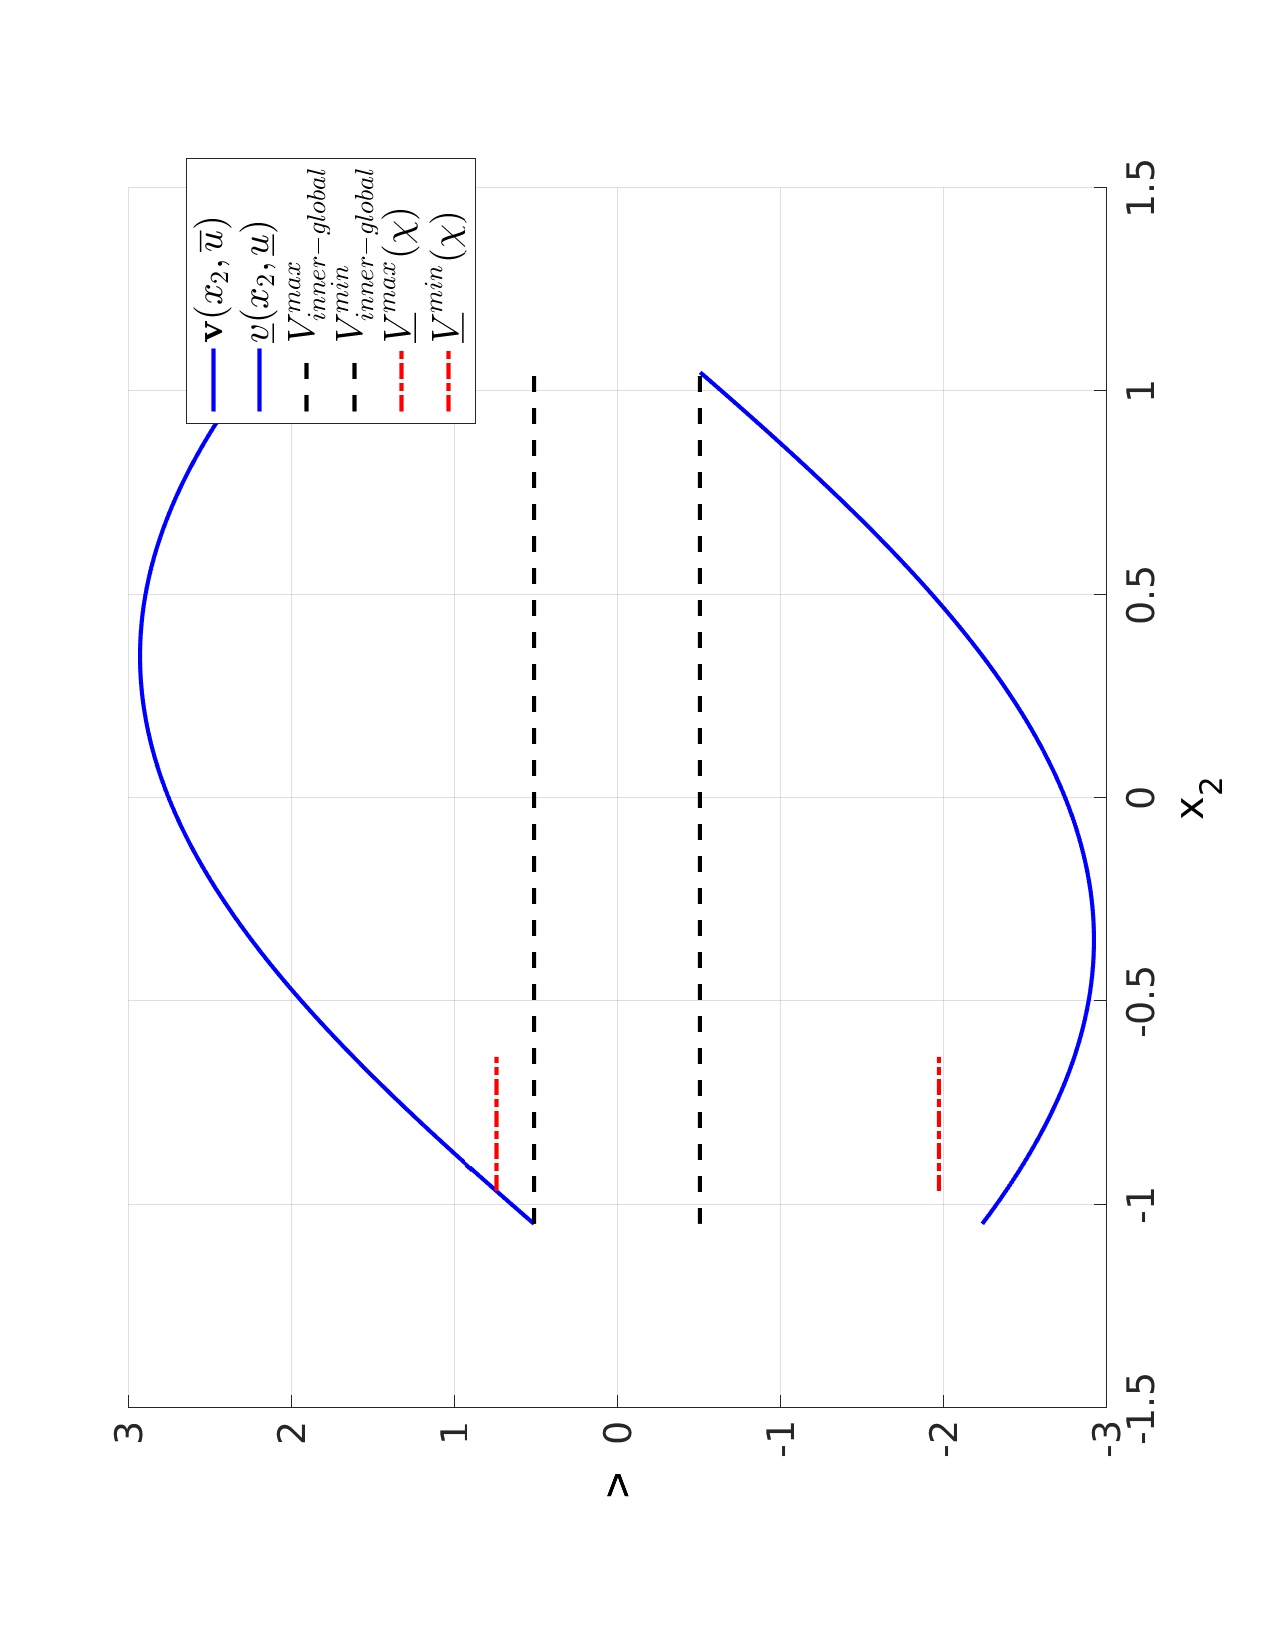
\includegraphics[angle=270,width=0.49\textwidth]{figs/InputToy.pdf}
\caption{The input limit sets and the true bounds for the running example}
\label{fig:err_bound_toy}
\end{figure}


\subsection{Computing the bounding error set and disturbance approximations online}

In Sec. \ref{sec:approx dist}, since the set $X_{k+j|k}$ is unknown and we only have access to a state estimate at time $k$, we use the online reachable set over-approximation of Sec. \ref{sec:x reach} to obtain $\oa{X}_{k+j|k}$.
Then it holds that 
\[\min_{x \in \oa{X}_{k+j|k} e \in E}M_i(x)e \leq \te_{k+j}(i) \leq \max_{x \in \oa{X}_{k+j|k}, e \in E} M_i(x)e\]

To make these computations easier, in the examples we use one last over-approximation to simplify the optimizations needed to calculate the component-wise bounds, specifically, we use 
\begin{eqnarray}
\label{eq:Etilde}
\sum_{\ell=1}^{n} \min_{x \in \oa{X}_{k+j|k}, e \in E} M_{i\ell}(x)e(\ell)  \leq \te_{k+j}(i) 
\nonumber 
\\
\leq \sum_{\ell=1}^{n} \max_{x \in \oa{X}_{k+j|k}, e \in E} M_{i\ell}(x)e(\ell)
\end{eqnarray}
where $M_{i\ell}$ is the $(i,\ell)^{th}$ element of matrix $M$.
Therefore we define the rectangular error set $\tE_{k+j|k}$ to be the set of vectors $e = [e_1,\ldots, e_{\dimZ}]^T$ satisfying \eqref{eq:Etilde}. The max and min involved in this can be now either be analyticaly computed, or be computed quickly at run-time using interval arithmetic (by computing the rectangular bounds on $\oa{X}_{k+j|k}$. While this adds a level of conservation, it guarantees us that we obtain an upper bound on the max and a lower bound on the min, which allows us to proceed without violating any assumptions.

While the sets $\tE_{k}$ over-approximate the mapped estimation error, we also need to calculate containing sets for the process noise $\hat{w}$.
Recall that for all $k,j$, 
$\hz_{k+j+1} = z_{k+j+1} + \te_{k+j+1} = Az_{k+j}+Bv_k+w_{k+j} + \te_{k+j+1} =  A(\hz_{k+j} - \te_{k+j}) + Bv_k + w_{k+j} + \te_{k+j+1} = A\hz_{k+j} + Bv_k + w_{k+j} + \te_{k+j+1} - A \te_{k+j} = A\hz_{k+j} + Bv_k + \hw_{k+j+1}$.

Therefore 
\begin{equation}
\label{eq:What}
\hw_{k+j+1} \in \What_{k+j+1|k} \defeq W \oplus \tE_{k+j+1|k} \oplus(-A\tE_{k+j|k})
\end{equation}

We also define the set $\tilde{E}_{max}$, which is necessary for the terminal constraints of Eq. \ref{eq:P_f_def}. $\tilde{E}_{max}$ represents the worst case error bound on the estimation error $\tilde{e}_k$, and is computed similar to Eq. \ref{eq:Etilde}, but over the entire set $X$ and not reachable subsets of it:

\begin{eqnarray}
\label{eq:EtildeMax}
\sum_{\ell=1}^{n} \min_{x \in X, e \in E} M_{i\ell}(x)e(\ell)  \leq \te_{k}(i) 
\nonumber 
\\
\leq \sum_{\ell=1}^{n} \max_{x \in X, e \in E} M_{i\ell}(x)e(\ell)
\end{eqnarray}

$\What_{max}$ is then defined as:
\begin{equation}
\What_{max} = W \oplus \tilde{E}_{max} \oplus (-A\tilde{E}_{max})
\end{equation}

For the running example, Fig. \ref{fig:err_bound_toy} shows the set $\tilde{E}_{max}$, the set $\tilde{E}$ computed over $\chi = [-\pi/4,0]\times[-0.9666,-0.6283]$. This shows that considering a reach set $\chi \subseteq X$ to compute the error bound results in less conservatism than using the worst case error bound. It also shows randomised realizations of the error for randomly selected $x \in \chi$ and $e \in E$, which are all contained in the bounding set $\tilde{E}_{\chi}$.

\begin{figure}
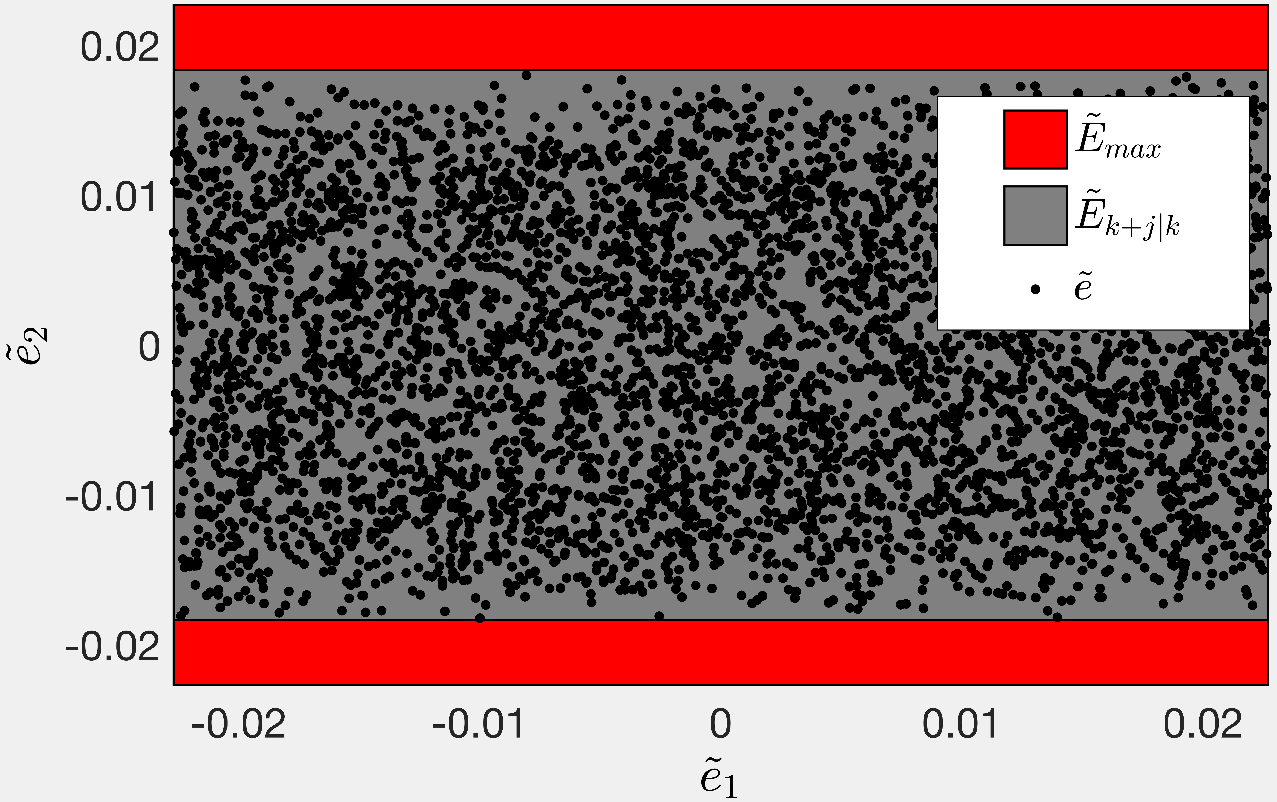
\includegraphics[angle=270,width=0.49\textwidth]{figs/Err_Bounds_toy.pdf}
\caption{The error sets $\tilde{E}_{max}$ and $\tilde{E}$ computed over the set $\chi$. Also shown are random realizations of the error $\tilde{e}$ for random $e \in E$ and $x \in \chi$.}
\label{fig:err_bound_toy}
\end{figure}

